\chapter{Types \& Characteristics}\label{ch:types_technologies_characteristics}

\glspl{ntn} are an emerging approach in the field of wireless communication that aims to expand network coverage beyond the reach of traditional terrestrial systems. By utilizing platforms such as satellites, \glspl{uav}, and \glspl{hap}, \glspl{ntn} can address the growing demand for global connectivity, particularly in remote or inaccessible areas.\ \glspl{ntn} offer a flexible and adaptable infrastructure, supporting a wide range of applications from disaster recovery to rural broadband access.

The following sections explore the various types of \glspl{ntn}, also referred as architectural models, highlighting their roles in enhancing communication networks, the benefits they offer, and the challenges they face. These architectures include platforms functioning as network users, relays, and base stations, along with mixed models that combine different approaches to maximize efficiency and coverage. The diagram of the different architectures of \gls{ntn} platforms according to their use case is shown in \cref{fig:ntn_platforms}.

\begin{figure}
  \begin{subfigure}{0.4\textheight}
    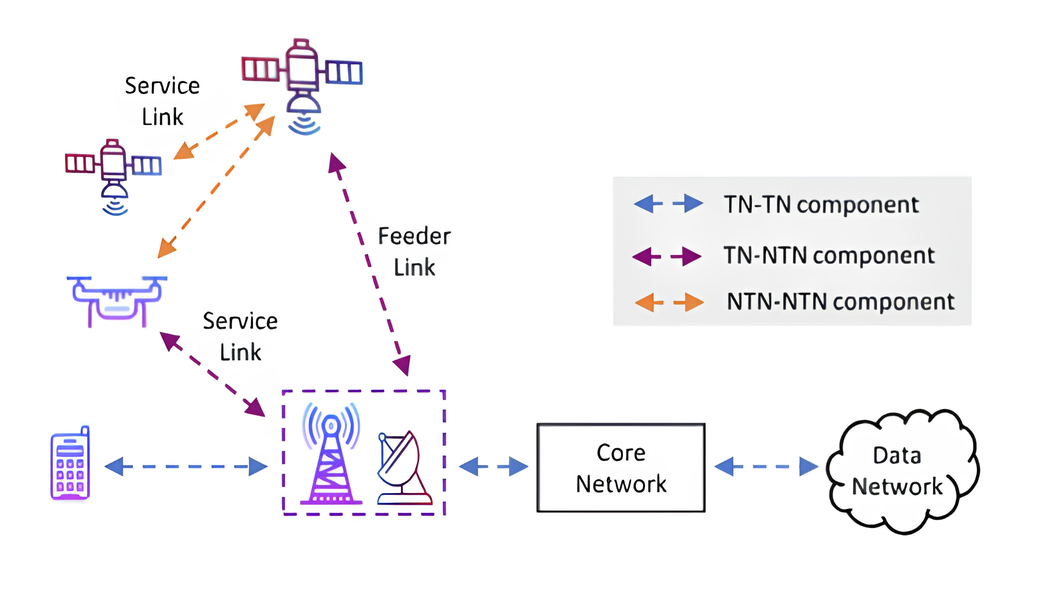
\includegraphics{ntn_use_case_platform_as_a_user.png}
    \caption{Diagram of NTN Platforms as Network Users where the NTN acts as another UE in the network.}\label{fig:ntn_platform_as_a_user}
  \end{subfigure}

  \begin{subfigure}{0.4\textheight}
    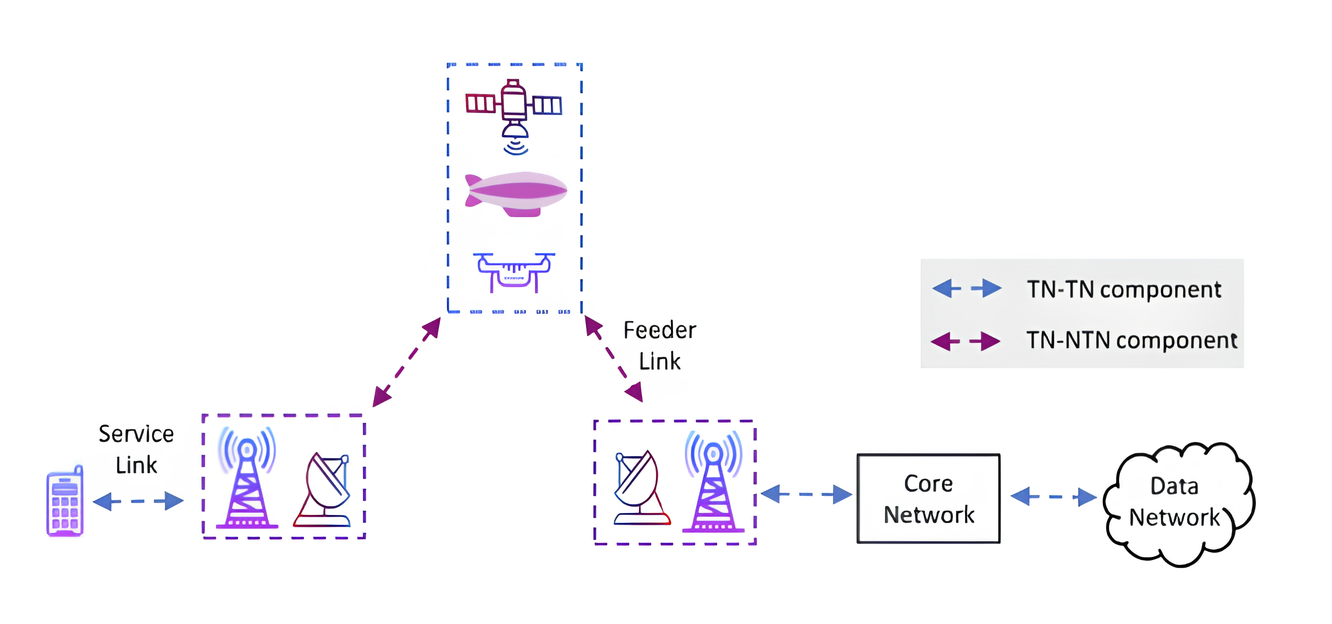
\includegraphics{ntn_use_case_platform_as_a_relay.png}
    \caption{Diagram of NTN Platforms as Relays where the NTN acts as a relay between the UE and the base station.}\label{fig:ntn_platform_as_a_relay}
  \end{subfigure}

  \begin{subfigure}{0.4\textheight}
    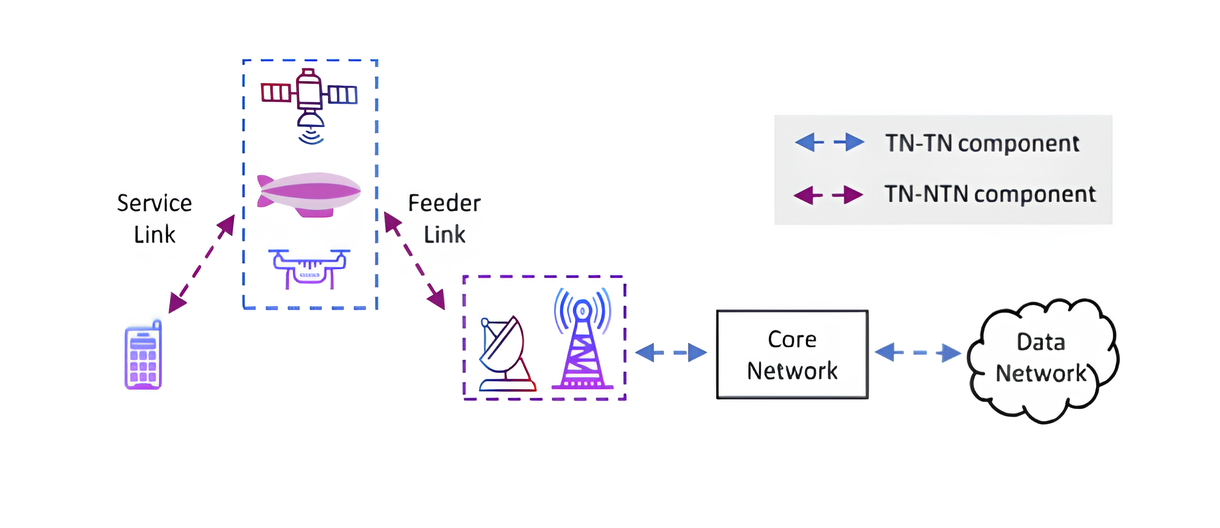
\includegraphics{ntn_use_case_platform_as_a_base_station.png}
    \caption{Diagram of NTN Platforms as Base Stations where the NTN acts as a base station for the UE.}\label{fig:ntn_platform_as_a_base_station}
  \end{subfigure}

  \begin{subfigure}{0.4\textheight}
    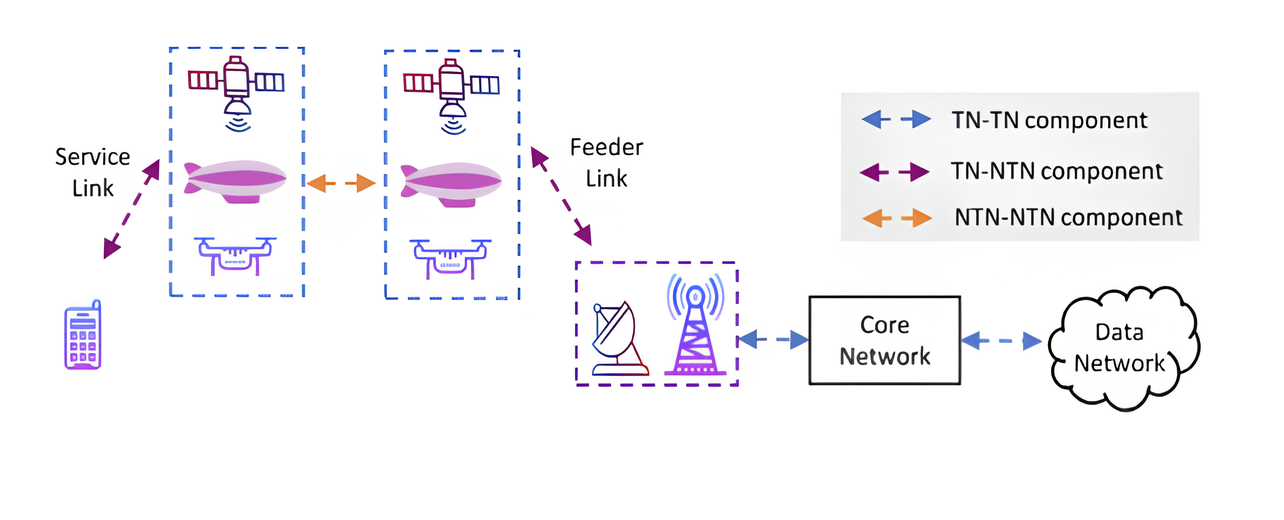
\includegraphics{ntn_use_case_platform_mixed.png}
    \caption{Diagram of Mixed Architecture Models where the NTN acts as a combination of the above.}\label{fig:mixed_architecture_models}
  \end{subfigure}

  \caption{Different architectures of NTN platforms according to their use case \autocite{evolution_ntn_from_5g_6g_survey}.}\label{fig:ntn_platforms}
\end{figure}

\section{NTN Platforms as Network Users}\label{sec:ntn_platform_as_a_user}

In this architecture, the \gls{ntn} platform operates similarly to a user device, or \gls{ue}, connecting to an existing terrestrial network as depicted in \cref{fig:ntn_platform_as_a_user}. This model is particularly relevant for platforms like satellites and \glspl{uav}, which need connectivity for data transmission. \glspl{uav}, for instance, can access terrestrial networks via base stations located on the ground.

A well-known example is the integration of \glspl{uav} into terrestrial networks. The \gls{3gpp} has identified \glspl{uav} as a unique category of \gls{ue} \autocite{muruganathan2019overview3gpprelease15study}, leading to research on how to address their specific connectivity challenges \autocite{uav_assisted_networks_challenges}. These challenges include maintaining stable connections during flight, managing potential interference, and ensuring service quality at various altitudes. By treating \glspl{uav} as network users, terrestrial infrastructure can support a broader range of communication needs, such as surveillance, logistics, and remote sensing.

Additionally, in scenarios where terrestrial control stations are unavailable or impractical, satellites can communicate directly with other satellites. This capability eliminates the need for extensive ground infrastructure, improving data transmission efficiency and making it particularly beneficial for space missions and remote observation activities.

\section{NTN Platforms as Relays}\label{sec:ntn_platform_as_a_relay}

\gls{ntn} platforms can also serve as relays, functioning as intermediaries that transmit signals between different components of the network, refer to \cref{fig:ntn_platform_as_a_relay}. This type of architecture can be categorized into two main configurations based on the relay's role within the network.

The first configuration involves backhaul connectivity \autocite{Elamassie2023FreeSO}, where the \gls{ntn} platform provides a link between a ground-based base station and the core network. This model is especially useful in remote or hard-to-reach areas where traditional backhaul solutions, such as fiber optic cables, are unavailable or too costly to install. By using satellites or \glspl{hap} as relays, terrestrial networks can be extended without requiring significant ground infrastructure.

In the second configuration, the \gls{ntn} platform acts as a direct relay between ground users and a terrestrial base station. This setup is particularly effective in environments where access to a base station is limited, such as densely populated urban areas or mountainous regions.\ \glspl{uav} or \gls{leo} satellites can serve as intermediary nodes, relaying user signals to the terrestrial network. This approach expands coverage and improves connectivity in areas where traditional infrastructure may not suffice \autocite{overview_on-5g-and-beyon-networks-with-uav}.

\section{NTN Platforms as Base Stations}\label{sec:ntn_platform_as_a_base_station}

\gls{ntn} platforms can also be configured to act as base stations, managing communication networks autonomously. Platforms equipped with advanced processing capabilities, such as regenerative payloads, can process signals onboard and provide connectivity without relying on ground-based infrastructure, as shown in \cref{fig:ntn_platform_as_a_base_station}. This architecture is particularly useful in scenarios where ground-based base stations are impractical or unavailable.

In the case of satellite-based base stations, satellites in \gls{leo} are equipped with onboard processors that handle tasks typically managed by terrestrial base stations, such as signal processing, traffic routing, and user management \autocite{leo_platforms_in_ntn}. This configuration is particularly well-suited for providing connectivity in remote regions, such as open seas, deserts, or disaster-stricken areas where ground infrastructure is impractical or unavailable.

\glspl{uav} can also function as temporary base stations, providing localized network coverage in specific areas. For example, \glspl{uav} equipped with \gls{5g} technology can deliver communication services during large-scale events, emergencies, or military operations. These \gls{uav}-based stations operate at lower altitudes than satellites, making them ideal for providing real-time, localized coverage with minimal delay.

\section{Mixed Architecture Models}\label{sec:mixed_architecture_models}

In real-world deployments, combining different architectural models is often necessary to create a more flexible and robust network infrastructure \autocite{hybrid_satellite_terrestrial_networks}, as shown in \cref{fig:mixed_architecture_models}. Mixed architecture models leverage the unique strengths of various \gls{ntn} platforms to optimize communication performance and coverage.

One example of a mixed architecture is a combination of \gls{leo} satellites and \glspl{uav}. In this configuration, a \gls{leo} satellite equipped with base station capabilities can work alongside \glspl{uav} acting as relays to extend coverage to ground users. The \glspl{uav}, operating at lower altitudes, enhance connectivity by relaying signals to the satellite, which then forwards the data to the core network. This approach ensures a broader coverage area and improved network performance.

Another example involves multi-tier satellite configurations \autocite{5g_allstar}, where satellites at different altitudes work together to provide comprehensive coverage. For instance, a \gls{geo} satellite can serve as a high-level backhaul link to the core network, while \gls{leo} satellites deliver low-latency connectivity to end users. This multi-tier approach combines the strengths of \gls{geo} and \gls{leo} satellites, offering both extensive coverage and low-latency communication.

Finally, \glspl{hap} can be integrated into \gls{ntn} networks to act as intermediary nodes between UAVs and satellites. In this configuration, \glspl{hap} receive data from \glspl{uav} below and transmit it to \gls{leo} satellites above, improving data transmission efficiency. This multi-hop communication strategy is particularly useful in complex environments where direct satellite or terrestrial communication is difficult.

\section{Characteristics of Non-Terrestrial Networks}\label{sec:characteristics_of_non_terrestrial_networks}

\glspl{ntn} offer several benefits, but they also present challenges. One of the primary advantages of \glspl{ntn} is their ability to extend network coverage to regions where terrestrial infrastructure is either unavailable or impractical \autocite{evolution_ntn_from_5g_6g_survey}.\ \glspl{ntn} can provide connectivity in remote areas, including oceans, mountainous regions, and locations affected by natural disasters. Platforms like \glspl{uav} and \glspl{hap} are especially useful in emergencies, as they can be quickly deployed to restore communication services and support disaster relief efforts.

In addition, \glspl{ntn} provide a flexible communication infrastructure by integrating different types of platforms. This adaptability makes \glspl{ntn} suitable for meeting the needs of diverse applications across various regions. Moreover,\ \glspl{ntn} are often more cost-effective than traditional networks, especially in sparsely populated areas where building extensive ground infrastructure would be prohibitively expensive.

However, \glspl{ntn} also face several challenges. Latency is a significant concern, especially in systems that rely on multiple satellite hops or satellite-to-satellite communication. High latency can affect the performance of real-time applications, such as voice or video communication. Signal interference is another issue, as multiple platforms operating at different altitudes and frequencies can lead to overlapping signals. Effective spectrum management is critical to maintaining service quality in \gls{ntn} deployments.

Power limitations, particularly for \glspl{uav} and certain \glspl{hap}, can restrict their operational duration \autocite{power_efficiency_uav}. Additionally, regulatory challenges, such as airspace management and frequency allocation, pose obstacles to the widespread deployment of \glspl{ntn}. For instance, \gls{uav}-based \gls{ntn} platforms must comply with international airspace regulations, while satellite-based \glspl{ntn} require coordination across different countries to ensure proper frequency usage.

\glspl{ntn} serve a variety of use cases across different sectors. In disaster recovery scenarios, \glspl{ntn} can be rapidly deployed to restore communication networks for emergency response teams \autocite{ntn_challenges_and_opportunities}.\ \glspl{ntn} are also valuable for environmental monitoring and remote sensing, providing continuous observation over large areas, such as forests, oceans, and agricultural lands. In the aviation and maritime sectors, \glspl{ntn} provide reliable connectivity for aircraft and ships, offering essential communication services in regions beyond terrestrial coverage. Finally, \glspl{ntn} play a crucial role in reducing the digital divide by delivering broadband internet access to rural and remote communities where traditional networks are not viable.

% Local Variables:
% jinx-local-words: "ntn uav ue"
% End:
